\RequirePackage{fix-cm}
%
\RequirePackage{amsmath}



%\documentclass{svjour3}                     % onecolumn (standard format)
%\documentclass[smallcondensed]{svjour3}     % onecolumn (ditto)
%\documentclass[smallextended]{svjour3}       % onecolumn (second format)
% \documentclass[twocolumn]{svjour3}          % twocolumn
%\documentclass[letterpaper, 12pt, twocolumn]{article}
\documentclass{article}
\usepackage[cm]{fullpage}
%\usepackage[margin=1in]{geometry}
\usepackage{amssymb}
\usepackage{graphicx}
\usepackage[utf8]{inputenc}
\usepackage{indentfirst}
%\usepackage{physics}
\newcommand{\me}{\mathrm{e}}
\usepackage{amsmath}

%\usepackage[monochrome]{color}

%\usepackage[round]{natbib}
%\usepackage{apacite}
\usepackage{url}


\PassOptionsToPackage{monochrome}{xcolor}

% For the flow charts
\usepackage{tikz}
\usetikzlibrary{
	external,
}
\tikzexternalize

\usetikzlibrary{shapes.geometric, arrows, calc, positioning}
\tikzstyle{startstop} = [rectangle, thick, rounded corners=2.5mm, minimum width=2cm, minimum height=5mm,text centered, draw=black]
\tikzstyle{io} = [trapezium, thick, trapezium left angle=70, trapezium right angle=110, text width=3.75cm, minimum height=0.5cm, text centered, draw=black]
\tikzstyle{process} = [rectangle, thick, minimum width=2.5cm, text width=4cm, minimum height=0.5cm, text centered, draw=black]
\tikzstyle{block} = [rectangle, thick, minimum width=0.5cm, minimum height=1cm, text centered, draw=black]
\tikzstyle{support} = [coordinate, join=by fuzzy]
\tikzstyle{decision} = [diamond, thick, minimum width=3cm, minimum height=1cm, text centered, draw=black]
\tikzstyle{dottedbox} = [rectangle, dotted, thick, minimum width=2.5cm, text width=2.8cm, minimum height=0.5cm, text centered, draw=black]
\tikzstyle{arrow} = [thick,->,>=stealth]
\tikzstyle{dottedarrow} = [thick, dotted,->,>=stealth]





\usepackage{pgfplots}
\usepgfplotslibrary{patchplots}
\pgfplotsset{compat=newest, samples=015} %Set this value to 65 for the final version
%\usepgfplotslibrary{dateplot} 


%\providecommand{\keywords}[1]{\textbf{\textit{Index terms---}} #1}

%\journalname{Journal of Science Education and Technology}

\begin{document}
	
	
	\title{Diagrams for the android app Control Toolbox (Continuous time)}
	\begin{figure}
		\centering
		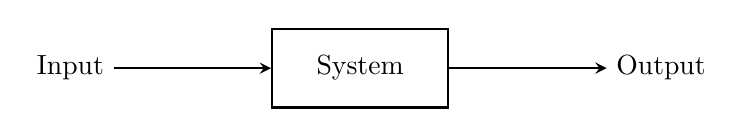
\begin{tikzpicture}[node distance = 10mm, auto]
		\node (Input) [align=center] {Input};
		\node (Plant) [block, text width = 2cm, right = 2cm of Input] {System};
		\node (Output) [right = of Plant, right = 2cm, align=center] {Output};
		\draw [arrow] (Input) -- (Plant);
		\draw [arrow] (Plant) -- (Output);
		\end{tikzpicture}
		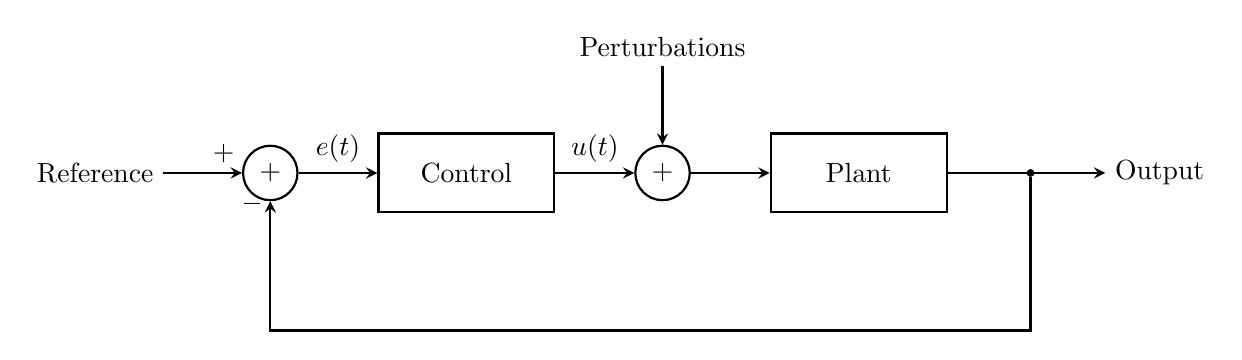
\begin{tikzpicture}[node distance = 10mm, auto]
		\node (Reference) [align=center] {Reference};
		\node (SummingPoint) [draw,circle, thick, right = of Reference]  {+};
		\node (Control) [block, text width = 2cm, right = of SummingPoint] {Control};
		\node (SummingPoint1) [draw,circle, thick, right = of Control]  {+};
		\node (Plant) [block, text width = 2cm, right = of SummingPoint1] {Plant};
		\node (PlantRight) [support, right = of Plant, right = 1cm, fill, circle,scale=0.3] {};
		\node (Output) [right = of Plant, right = 2cm, align=center] {Output};
		\node (Perturbations) [align=center, above = of SummingPoint1] {Perturbations};
		\draw [arrow] (Reference) -- node[anchor=south west]{+}(SummingPoint);
		\draw [arrow] (SummingPoint) -- node[anchor=south]{$e(t)$}(Control);
		\draw [arrow] (Control) -- node[anchor=south]{$u(t)$}(SummingPoint1);
		\draw [arrow] (SummingPoint1) -- (Plant);
		\draw [arrow] (Plant) -- (Output);
		\draw [arrow] (PlantRight) -- +(0, -2) -| (SummingPoint) node[below = 2mm, anchor=north east]{\bf\textendash};
		\draw [arrow] (Perturbations) -- (SummingPoint1);
		\end{tikzpicture}
		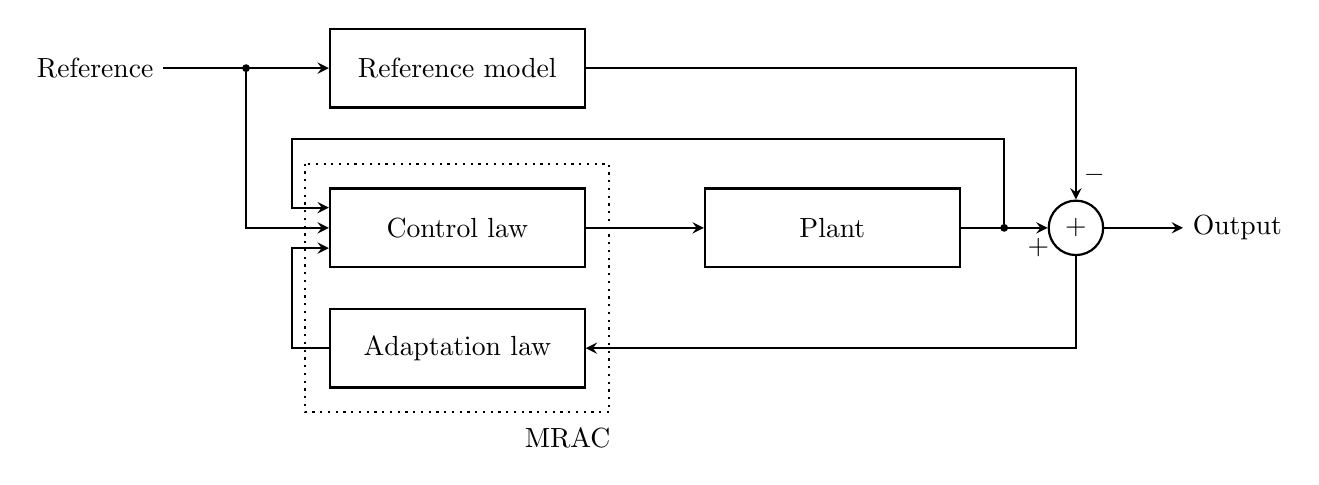
\begin{tikzpicture}[node distance = 10mm, auto]
		\node (Reference) [align=center] {Reference};
		\node (ReferenceRight) [support, right = of Reference, fill,circle,scale=0.3] {};
		\node (RefModel) [block, text width = 3cm, right = of ReferenceRight] {Reference model};
		\node (Control) [block, text width = 3cm, below = of RefModel] {Control law};
		\node (Adaptation) [block, text width = 3cm, below = of Control, below = 5mm] {Adaptation law};
		\draw[thick, dotted] ($(Control.north west)+(-0.3,0.3)$)  rectangle ($(Adaptation.south east)+(0.3,-0.3)$)  (60mm, -47mm) node[]{MRAC};
		\node (Plant) [block, text width = 3cm, right = 15mm of Control] {Plant};
		\node (PlantRight) [support, right = of Plant, right = 5mm, fill,circle,scale=0.3] {};
		\node (SummingPoint) [draw,circle, thick, right = 25mm of PlantRight, right = 5mm ]  {+};
		\node (Output) [right = of SummingPoint, align=center] {Output};
		
		\path (Reference.east) -- (Reference.east) coordinate[pos=05] (Reference1);
		\path (Control.west) -- (Control.north west) coordinate[pos=-	0.5] (Control1);
		\path (Control.west) -- (Control.north west) coordinate[pos=+0.5] (Control2);
		
		\draw [arrow] (Reference) -- node[anchor=south west]{}(RefModel);
		\draw [arrow] (ReferenceRight) |- (Control);
		\draw [arrow] (RefModel) -| node[pos=0.85, anchor = north west]{\bf\textendash}(SummingPoint);
		\draw [arrow] (Control) -- node [] {}(Plant);
		\draw [arrow] (Plant) -- node[pos=0.65, anchor=north west]{+}
		(SummingPoint);
		\draw [arrow] (SummingPoint) -- (Output);
		\draw [arrow] (SummingPoint) |- node[pos=0.98, anchor=north west]{} (Adaptation);
		\draw [arrow] (Adaptation) -| node [pos=1, anchor=north east]{}(25mm,-30mm) |- (Control1);
		\draw [arrow] (PlantRight) |- (25mm,-9mm) |- (Control2);		
		\end{tikzpicture}
		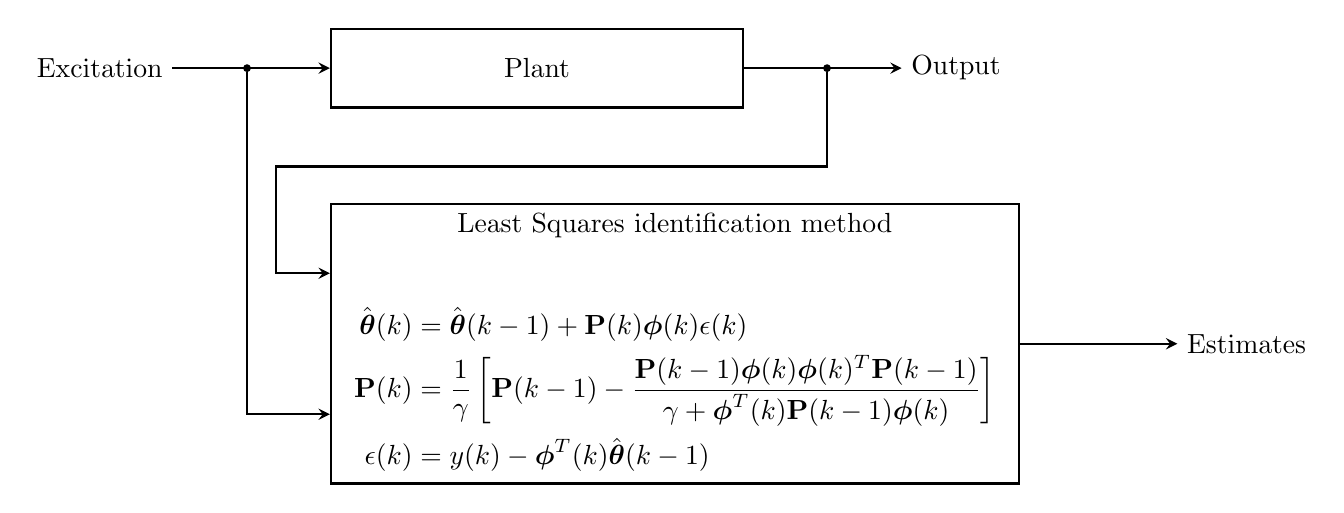
\begin{tikzpicture}[node distance = 10mm, auto]
		\node (Excitation) [align=center] {Excitation};
		\node (Plant) [block, text width = 5cm, right = of Excitation, right = 2cm] {Plant};
		\node (PlantRight) [support, right = of Plant, right = 1cm, fill,circle,scale=0.3] {};
		\node (PlantLeft) [support, left = of Plant, left = 1cm, fill,circle,scale=0.3] {};
		\node (Identification) [block, text width = 8.5cm, below = 3.5 of Plant.west, anchor=west] {Least Squares identification method
			\\[0.1cm]
			\begin{align}
			\hat{\boldsymbol{ \theta}}(k) &=\hat{\boldsymbol{ \theta}}(k-1)+\mathbf{P}(k)\boldsymbol{ \phi}(k)\epsilon(k) \nonumber\\ 
			\mathbf{P}(k) &=\dfrac{1}{\gamma}\left[\mathbf{P}(k-1)-\dfrac{\mathbf{P}(k-1)\boldsymbol{ \phi}(k)\boldsymbol{ \phi}(k)^{T}\mathbf{P}(k-1)}{\gamma+\boldsymbol{ \phi}^{T}(k)\mathbf{P}(k-1)\boldsymbol{ \phi}(k)}\right] \nonumber\\ 
			\epsilon(k) &=y(k)-\boldsymbol{ \phi}^{T}(k)\hat{\boldsymbol{ \theta}}(k-1) \nonumber 
			\end{align}
		};
		\node (Output) [right = of Plant, right = 2cm, align=center] {Output};
		\node (CapValues) [right = of Identification, right = 2cm, align=center] {Estimates};
		\path (Excitation.east) -- (Excitation.north east) coordinate[pos=0.5] (Reference1);
		\path (Identification.west) -- (Identification.north west) coordinate[pos=0.5] (Identification1);
		\path (Identification.west) -- (Identification.north west) coordinate[pos=-0.5] (Identification2);
		\draw [arrow] (Excitation) -- (Plant);
		\draw [arrow] (Plant) -- (Output);
		\draw [arrow] (PlantRight) -- +(0, -1.25) -| +(-7,-1.25) |- (Identification1);
		\draw [arrow] (PlantLeft) |- (Identification2);
		\draw [arrow] (Identification) -- (CapValues);
		\end{tikzpicture}
		\caption{Background for the app}
		\label{Fig:Background}
	\end{figure}

	\begin{figure}
		\centering
		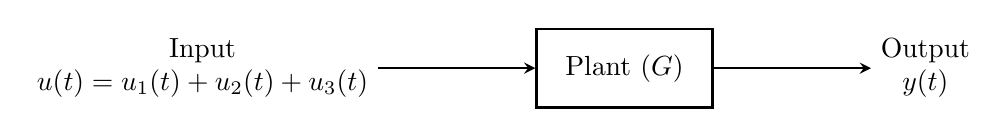
\begin{tikzpicture}[node distance = 10mm, auto]
		\node (Input) [align=center] {Input\\$u(t)=u_1(t)+u_2(t)+u_3(t)$};
		\node (Plant) [block, text width = 2cm, right = 2cm of Input] {Plant ($G$)};
		\node (Output) [right = of Plant, right = 2cm, align=center] {Output\\$y(t)$};
		\draw [arrow] (Input) -- (Plant);
		\draw [arrow] (Plant) -- (Output);
		\end{tikzpicture}
		\caption{Open loop system}
		\label{Fig:OpenLoop}
	\end{figure}
	
	
	\begin{figure}
		\centering
		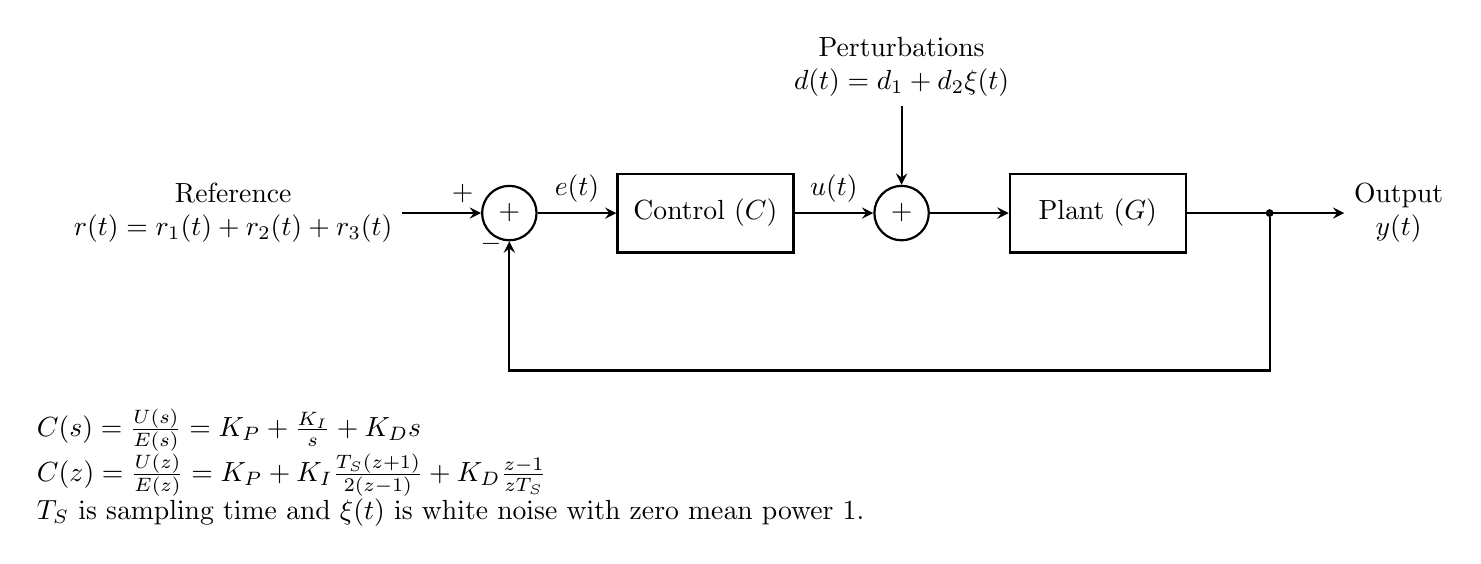
\begin{tikzpicture}[node distance = 10mm, auto]
		\node (Reference) [align=center] {Reference\\$r(t)=r_1(t)+r_2(t)+r_3(t)$};
		\node (SummingPoint) [draw,circle, thick, right = of Reference]  {+};
		\node (Control) [block, text width = 2cm, right = of SummingPoint] {Control ($C$)};
		\node (SummingPoint1) [draw,circle, thick, right = of Control]  {+};
		\node (Plant) [block, text width = 2cm, right = of SummingPoint1] {Plant ($G$)};
		\node (PlantRight) [support, right = of Plant, right = 1cm, fill, circle,scale=0.3] {};
		\node (Output) [right = of Plant, right = 2cm, align=center] {Output\\$y(t)$};
		\node (Perturbations) [align=center, above = of SummingPoint1] {Perturbations\\$d(t)=d_1+d_2\xi(t)$};
		\draw [arrow] (Reference) -- node[anchor=south west]{+}(SummingPoint);
		\draw [arrow] (SummingPoint) -- node[anchor=south]{$e(t)$}(Control);
		\draw [arrow] (Control) -- node[anchor=south]{$u(t)$}(SummingPoint1);
		\draw [arrow] (SummingPoint1) -- (Plant);
		\draw [arrow] (Plant) -- (Output);
		\draw [arrow] (PlantRight) -- +(0, -2) -| (SummingPoint) node[below = 2mm, anchor=north east]{\bf\textendash};
		\draw [arrow] (Perturbations) -- (SummingPoint1);
		\node (Equation000) [text width = 12cm, below = 2cm of SummingPoint, align = left] {
			$C(s) = \frac{U(s)}{E(s)} = K_P + \frac{K_I}{s} + K_Ds$\\
			$C(z) = \frac{U(z)}{E(z)} = K_P + K_I\frac{T_S(z+1)}{2(z-1)} + K_D\frac{z-1}{zT_S}$\\
			$T_S$ is sampling time and $\xi(t)$ is white noise with zero mean power 1.
		};
		\end{tikzpicture}
		\caption{Closed loop system with a PID Controller}
		\label{Fig:PID}
	\end{figure}
	
	\begin{figure}
		\centering
		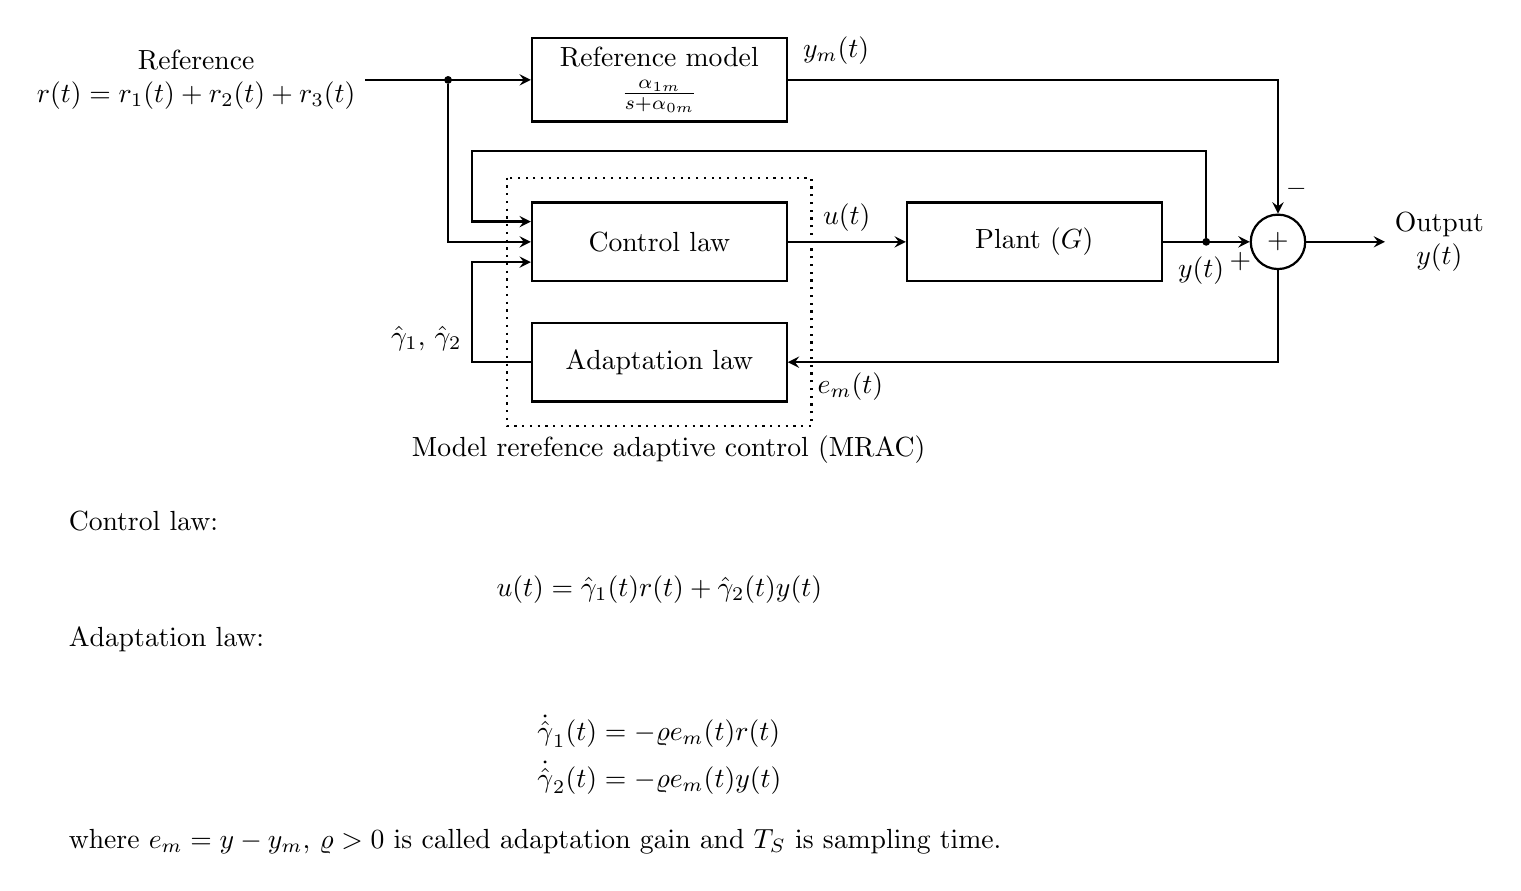
\begin{tikzpicture}[node distance = 10mm, auto]
		\node (Reference) [align=center] {Reference\\$r(t)=r_1(t)+r_2(t)+r_3(t)$};
		\node (ReferenceRight) [support, right = of Reference, fill,circle,scale=0.3] {};
		\node (RefModel) [block, text width = 3cm, right = of ReferenceRight] {Reference model\\ $\frac{\alpha_{1m}}{s + \alpha_{0m}}$};
		\node (Control) [block, text width = 3cm, below = of RefModel] {Control law};
		\node (Adaptation) [block, text width = 3cm, below = of Control, below = 5mm] {Adaptation law};
		\draw[thick, dotted] ($(Control.north west)+(-0.3,0.3)$)  rectangle ($(Adaptation.south east)+(0.3,-0.3)$)  (60mm, -47mm) node[]{Model rerefence adaptive control (MRAC)};
		\node (Plant) [block, text width = 3cm, right = 15mm of Control] {Plant ($G$)};
		\node (PlantRight) [support, right = of Plant, right = 5mm, fill,circle,scale=0.3] {};
		\node (SummingPoint) [draw,circle, thick, right = 25mm of PlantRight, right = 5mm ]  {+};
		\node (Output) [right = of SummingPoint, align=center] {Output\\$y(t)$};
		
		\path (Reference.east) -- (Reference.east) coordinate[pos=05] (Reference1);
		\path (Control.west) -- (Control.north west) coordinate[pos=-0.5] (Control1);
		\path (Control.west) -- (Control.north west) coordinate[pos=+0.5] (Control2);
		
		\draw [arrow] (Reference) -- node[anchor=south west]{}(RefModel);
		\draw [arrow] (ReferenceRight) |- (Control);
		\draw [arrow] (RefModel) -| node[pos=0.85, anchor = north west]{\bf\textendash}(SummingPoint);
		\draw [arrow] (Control) -- node [] {$u(t)$}(Plant);
		\draw [arrow] (Plant) -- node[pos=0.65, anchor=north west]{+}
		(SummingPoint);
		\draw [arrow] (SummingPoint) -- (Output);
		\draw [arrow] (SummingPoint) |- node[pos=0.98, anchor=north west]{$e_m(t)$} (Adaptation);
		\draw [arrow] (Adaptation) -| node [pos=1, anchor=north east]{${\hat{\gamma }}_{1}$, ${\hat{\gamma }}_{2}$}(35mm,-30mm) |- (Control1);
		\draw [arrow] (PlantRight) |- (35mm,-9mm) |- (Control2);

		\node [above right = 0.1 of RefModel.east]{$y_m(t)$};
		\node [below right = 0.1 of Plant.east]{$y(t)$};

		
		\node (Equation000) [text width = 15cm, below = 1.25cm of Adaptation, align = left] {
			Control law:\\
			\[u(t)={{\hat{\gamma }}_{1}}(t)r(t)+{{\hat{\gamma }}_{2}}(t)y(t)\]	
			Adaptation law:\\
			\begin{align}
				{{\dot{\hat{\gamma }}}_{1}}(t)&=-\varrho {{e}_{m}}(t)r(t)\nonumber\\
				{{\dot{\hat{\gamma }}}_{2}}(t)&=-\varrho {{e}_{m}}(t)y(t)\nonumber
			\end{align}
			where $e_m = y-y_m$, $\varrho>0$ is called adaptation gain and $T_S$ is sampling time.
		};
		\end{tikzpicture}
		\caption{Adaptive control}
		\label{Fig:AdaptiveControlFirstOrder}
	\end{figure}
	
	\begin{figure}
		\centering
		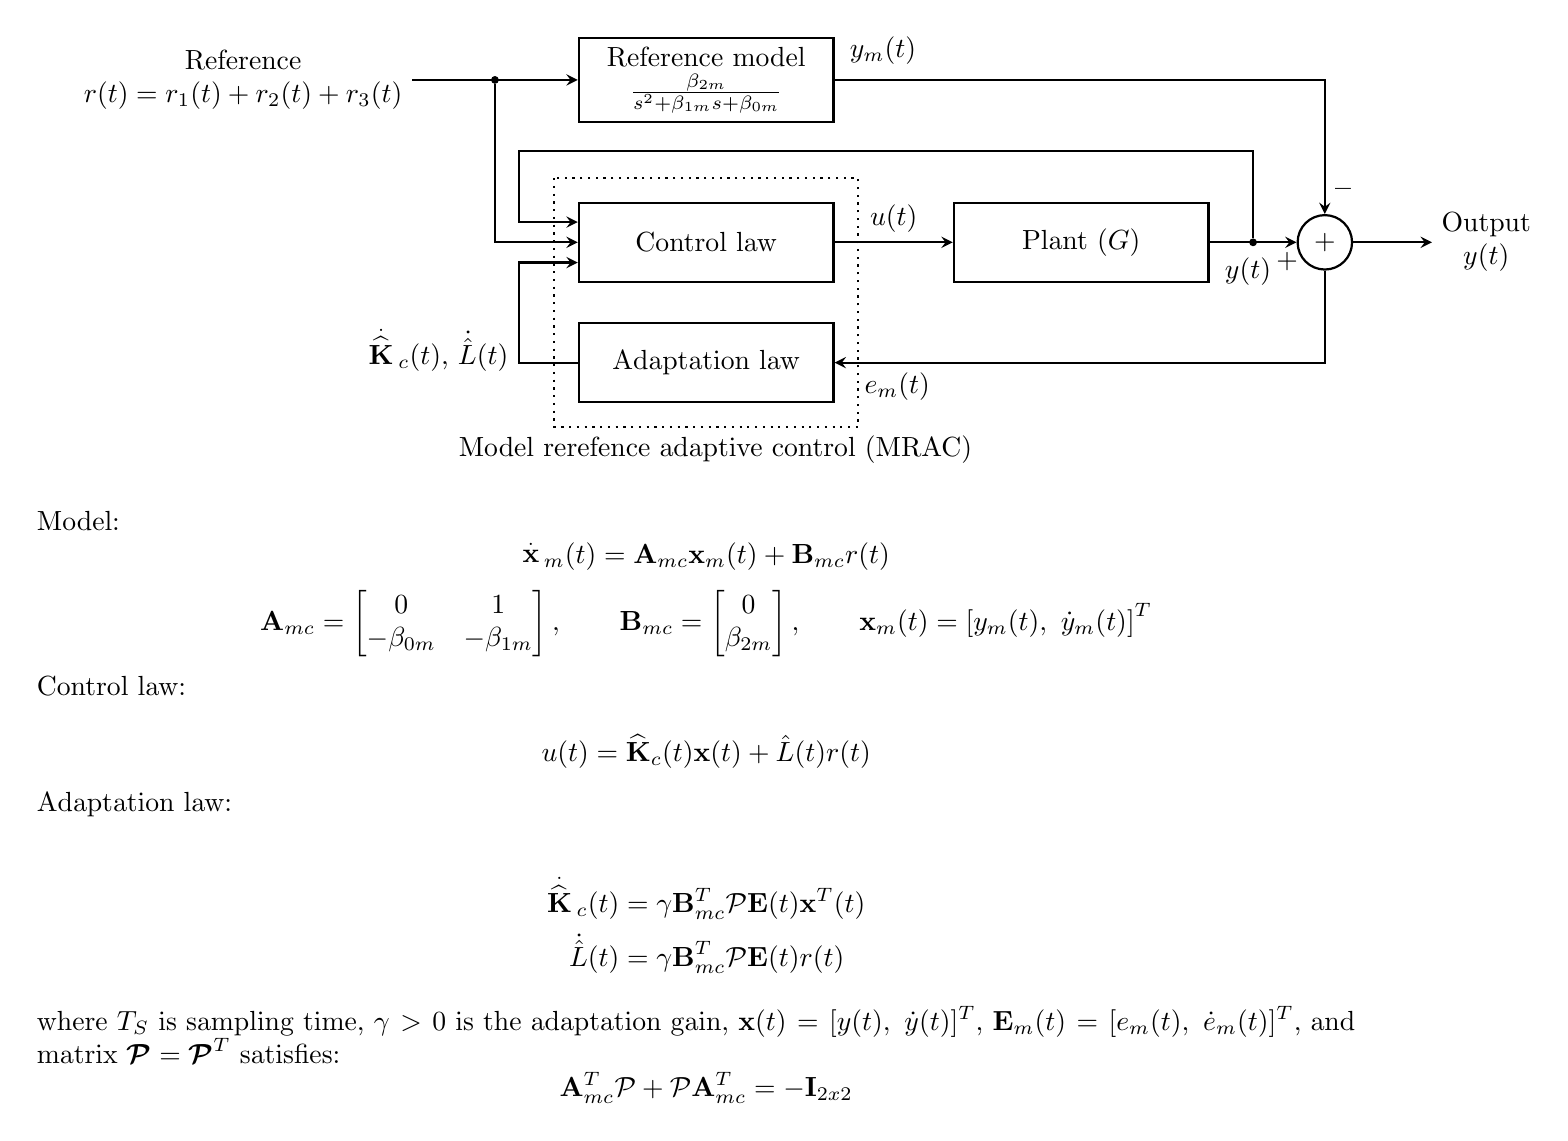
\begin{tikzpicture}[node distance = 10mm, auto]
		\node (Reference) [align=center] {Reference\\$r(t)=r_1(t)+r_2(t)+r_3(t)$};
		\node (ReferenceRight) [support, right = of Reference, fill,circle,scale=0.3] {};
		\node (RefModel) [block, text width = 3cm, right = of ReferenceRight] {Reference model\\ $\frac{\beta_{2m}}{s^2 + \beta_{1m}s + \beta_{0m}}$};
		\node (Control) [block, text width = 3cm, below = of RefModel] {Control law};
		\node (Adaptation) [block, text width = 3cm, below = of Control, below = 5mm] {Adaptation law};
		\draw[thick, dotted] ($(Control.north west)+(-0.3,0.3)$)  rectangle ($(Adaptation.south east)+(0.3,-0.3)$)  (60mm, -47mm) node[]{Model rerefence adaptive control (MRAC)};
		\node (Plant) [block, text width = 3cm, right = 15mm of Control] {Plant ($G$)};
		\node (PlantRight) [support, right = of Plant, right = 5mm, fill,circle,scale=0.3] {};
		\node (SummingPoint) [draw,circle, thick, right = 25mm of PlantRight, right = 5mm ]  {+};
		\node (Output) [right = of SummingPoint, align=center] {Output\\$y(t)$};
		
		\path (Reference.east) -- (Reference.east) coordinate[pos=05] (Reference1);
		\path (Control.west) -- (Control.north west) coordinate[pos=-0.5] (Control1);
		\path (Control.west) -- (Control.north west) coordinate[pos=+0.5] (Control2);
		
		\draw [arrow] (Reference) -- node[anchor=south west]{}(RefModel);
		\draw [arrow] (ReferenceRight) |- (Control);
		\draw [arrow] (RefModel) -| node[pos=0.85, anchor = north west]{\bf\textendash}(SummingPoint);
		\draw [arrow] (Control) -- node [] {$u(t)$}(Plant);
		\draw [arrow] (Plant) -- node[pos=0.65, anchor=north west]{+}
		(SummingPoint);
		\draw [arrow] (SummingPoint) -- (Output);
		\draw [arrow] (SummingPoint) |- node[pos=0.98, anchor=north west]{$e_m(t)$} (Adaptation);
		\draw [arrow] (Adaptation) -| node [pos=1, anchor=north east]{${{\overset{.}{\mathop{\widehat{\mathbf{K}}}}\,}_{c}}(t)$, $\dot{\hat{L}}(t)$}(35mm,-30mm) |- (Control1);
		\draw [arrow] (PlantRight) |- (35mm,-9mm) |- (Control2);
		
		\node [above right = 0.1 of RefModel.east]{$y_m(t)$};
		\node [below right = 0.1 of Plant.east]{$y(t)$};
		
		
		\node (Equation000) [text width = 17cm, below = 1.25cm of Adaptation, align = left] {
			Model:
			\[{{\overset{.}{\mathop{\mathbf{x}}}\,}_{m}}(t)={{{\mathbf{A}}}_{mc}}{{\mathbf{x}}_{m}}(t)+{{{\mathbf{B}}}_{mc}}r(t)\]
			\[{{\mathbf{A}}_{mc}}=\left[ \begin{matrix}
			0 & 1  \\
			-{{\beta }_{0m}} & -{{\beta }_{1m}}  \\
			\end{matrix} \right],\qquad {{\mathbf{B}}_{mc}}=\left[ \begin{matrix}
			0  \\
			{{\beta }_{2m}}  \\
			\end{matrix} \right],\qquad {{\mathbf{x}}_{m}}(t)={{[{{y}_{m}}(t),\ {{\dot{y}}_{m}}(t)]}^{T}}\]
			
			Control law:\\
			\[u(t)={{\widehat{\mathbf{K}}}_{c}}(t)\mathbf{x}(t)+\hat{L}(t)r(t)\]	
			Adaptation law:\\
			\begin{align}
			{{\overset{.}{\mathop{\widehat{\mathbf{K}}}}\,}_{c}}(t) &=\gamma \mathbf{B}_{mc}^{T}\mathcal{P}\mathbf{E}(t){{\mathbf{x}}^{T}}(t)\nonumber\\
			\dot{\hat{L}}(t)&=\gamma \mathbf{B}_{mc}^{T}\mathcal{P}\mathbf{E}(t)r(t)\nonumber
			\end{align}
			where $T_S$ is sampling time, $\gamma>0$ is the adaptation gain, $\mathbf{x}(t)=[y(t), \ \dot{y}(t)]^{T}$, $\mathbf{E}_{m}(t)=[e_{m}(t), \ \dot{e}_{m}(t)]^{T}$, and matrix $\boldsymbol{\mathcal{P}}=\boldsymbol{\mathcal{P}}^{T}$  satisfies:
			\[\mathbf{A}_{mc}^{T}\mathcal{P}+\mathcal{P}\mathbf{A}_{mc}^{T}=-{{\mathbf{I}}_{2x2}}\]
			
		};
		\end{tikzpicture}
		\caption{Adaptive control}
		\label{Fig:AdaptiveControlSecondOrder}
	\end{figure}

	\begin{figure}
		\centering
		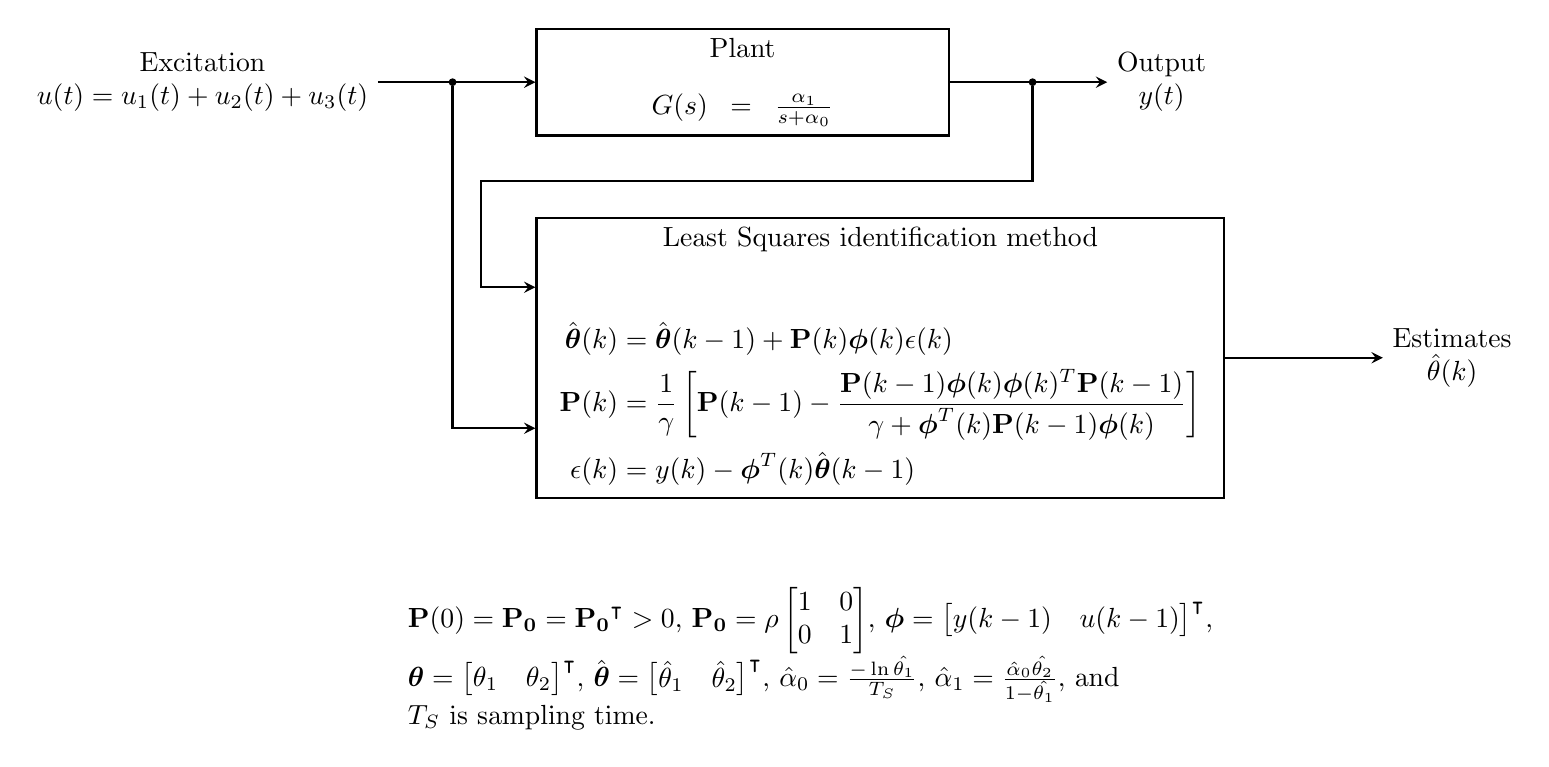
\begin{tikzpicture}[node distance = 10mm, auto]
		\node (Excitation) [align=center] {Excitation\\$u(t)=u_1(t)+u_2(t)+u_3(t)$};
		\node (Plant) [block, text width = 5cm, right = of Excitation, right = 2cm] {Plant \\[0.3cm] $G(s) = \frac{\alpha_1}{s+\alpha_0}$};
		\node (PlantRight) [support, right = of Plant, right = 1cm, fill,circle,scale=0.3] {};
		\node (PlantLeft) [support, left = of Plant, left = 1cm, fill,circle,scale=0.3] {};
		\node (Identification) [block, text width = 8.5cm, below = 3.5 of Plant.west, anchor=west] {Least Squares identification method
			\\[0.1cm]
			\begin{align}
			\hat{\boldsymbol{ \theta}}(k) &=\hat{\boldsymbol{ \theta}}(k-1)+\mathbf{P}(k)\boldsymbol{ \phi}(k)\epsilon(k) \nonumber\\ 
			\mathbf{P}(k) &=\dfrac{1}{\gamma}\left[\mathbf{P}(k-1)-\dfrac{\mathbf{P}(k-1)\boldsymbol{ \phi}(k)\boldsymbol{ \phi}(k)^{T}\mathbf{P}(k-1)}{\gamma+\boldsymbol{ \phi}^{T}(k)\mathbf{P}(k-1)\boldsymbol{ \phi}(k)}\right] \nonumber\\ 
			\epsilon(k) &=y(k)-\boldsymbol{ \phi}^{T}(k)\hat{\boldsymbol{ \theta}}(k-1) \nonumber 
			\end{align}
		};
		\node (Output) [right = of Plant, right = 2cm, align=center] {Output\\$y(t)$};
		\node (CapValues) [right = of Identification, right = 2cm, align=center] {Estimates\\$\hat{\theta}(k)$};
		\path (Excitation.east) -- (Excitation.north east) coordinate[pos=0.5] (Reference1);
		\path (Identification.west) -- (Identification.north west) coordinate[pos=0.5] (Identification1);
		\path (Identification.west) -- (Identification.north west) coordinate[pos=-0.5] (Identification2);
		\draw [arrow] (Excitation) -- (Plant);
		\draw [arrow] (Plant) -- (Output);
		\draw [arrow] (PlantRight) -- +(0, -1.25) -| +(-7,-1.25) |- (Identification1);
		\draw [arrow] (PlantLeft) |- (Identification2);
		\draw [arrow] (Identification) -- (CapValues);
		\node (Equation000) [text width = 12cm, below = 1cm of Identification, align = left] {
			$\mathbf{P}(0) = \mathbf{P_0} = \mathbf{P_0}^\intercal>0$, $\mathbf{P_0} = \rho
			\begin{bmatrix}
			1 & 0 \\
			0 & 1
			\end{bmatrix}$,
			$\boldsymbol{\phi} = \begin{bmatrix}
			y(k-1) &
			u(k-1)
			\end{bmatrix}^\intercal$, \\
			$\boldsymbol{\theta} = \begin{bmatrix}
			\theta_1 &
			\theta_2
			\end{bmatrix}^\intercal$,
			$\hat{\boldsymbol{\theta}} = \begin{bmatrix}
			\hat{\theta}_1 &
			\hat{\theta}_2
			\end{bmatrix}^\intercal$,
			$\hat{\alpha}_0 = \frac{-\ln{\hat{\theta_1}}}{T_S}$,
			$\hat{\alpha}_1 = \frac{\hat{\alpha}_0\hat{\theta_2}}{1-\hat{\theta_1}}$, and \\$T_S$ is sampling time.
		};
		\end{tikzpicture}
		\caption{First order system identification}
		\label{Fig:FirstOrderIdentification}
	\end{figure}
	
	\begin{figure}
		\centering
		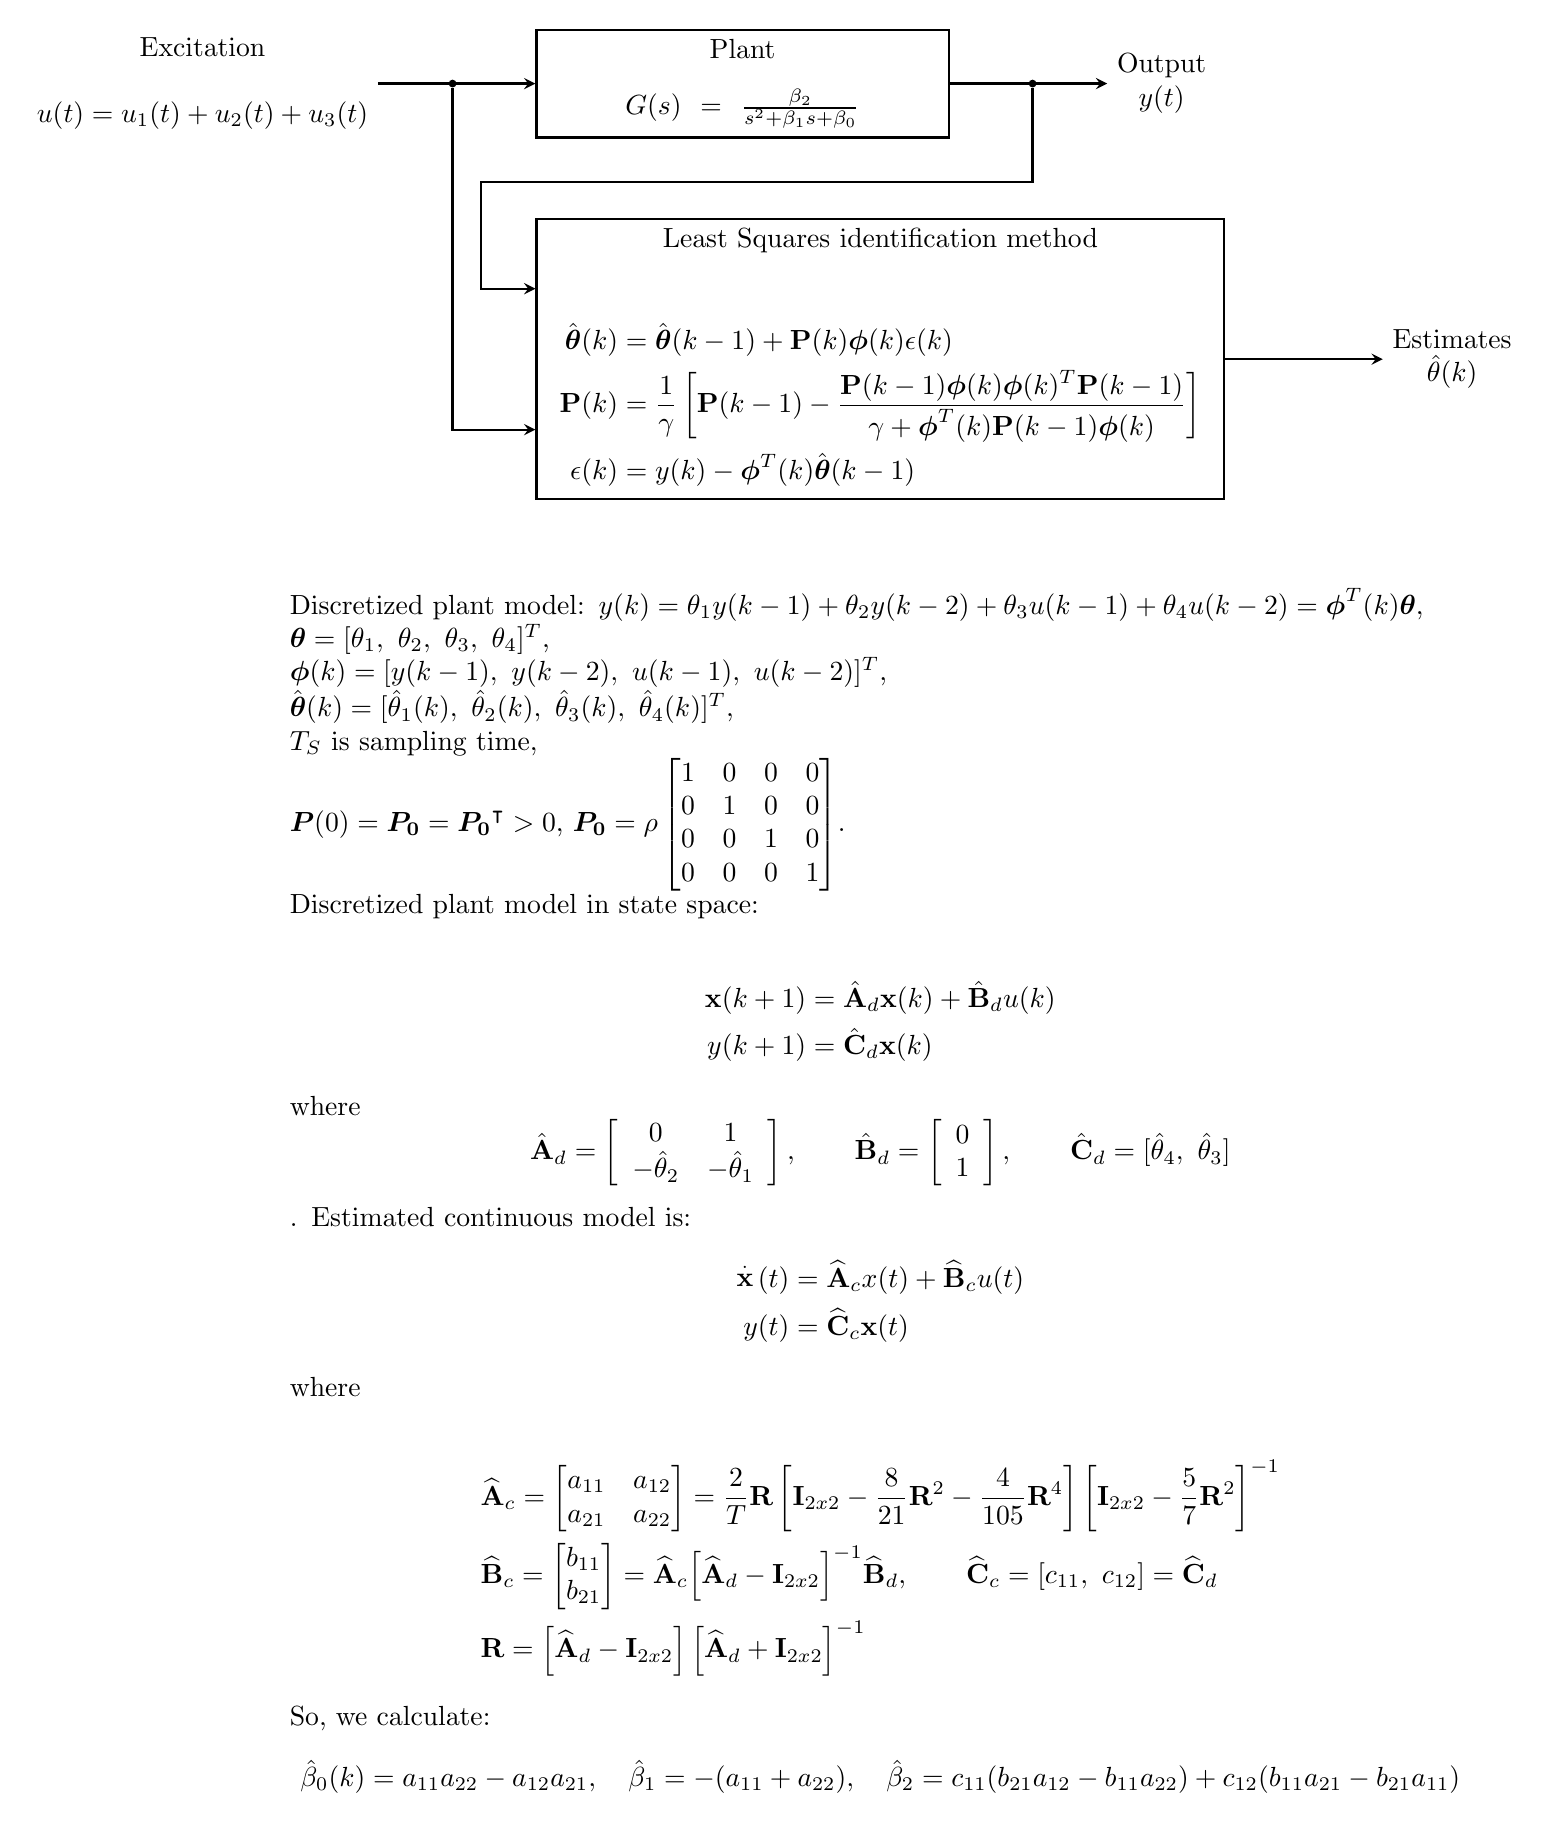
\begin{tikzpicture}[node distance = 10mm, auto]
		\node (Excitation) [align=center] {Excitation\\\\$u(t)=u_1(t)+u_2(t)+u_3(t)$};
		\node (Plant) [block, text width = 5cm, right = of Excitation, right = 2cm] {Plant \\[0.3cm] $G(s) = \frac{\beta_2}{s^2 + \beta_1s + \beta_0}$};
		\node (PlantRight) [support, right = of Plant, right = 1cm, fill,circle,scale=0.3] {};
		\node (PlantLeft) [support, left = of Plant, left = 1cm, fill,circle,scale=0.3] {};
		\node (Identification) [block, text width = 8.5cm, below = 3.5 of Plant.west, anchor=west] {Least Squares identification method
			\\[0.1cm]
			\begin{align}
			\hat{\boldsymbol{ \theta}}(k) &=\hat{\boldsymbol{ \theta}}(k-1)+\mathbf{P}(k)\boldsymbol{ \phi}(k)\epsilon(k) \nonumber\\ 
			\mathbf{P}(k) &=\dfrac{1}{\gamma}\left[\mathbf{P}(k-1)-\dfrac{\mathbf{P}(k-1)\boldsymbol{ \phi}(k)\boldsymbol{ \phi}(k)^{T}\mathbf{P}(k-1)}{\gamma+\boldsymbol{ \phi}^{T}(k)\mathbf{P}(k-1)\boldsymbol{ \phi}(k)}\right] \nonumber\\ 
			\epsilon(k) &=y(k)-\boldsymbol{ \phi}^{T}(k)\hat{\boldsymbol{ \theta}}(k-1) \nonumber 
			\end{align}
		};
		\node (Output) [right = of Plant, right = 2cm, align=center] {Output\\$y(t)$};
		\node (CapValues) [right = of Identification, right = 2cm, align=center] {Estimates\\$\hat{\theta}(k)$};
		\path (Excitation.east) -- (Excitation.north east) coordinate[pos=0.5] (Reference1);
		\path (Identification.west) -- (Identification.north west) coordinate[pos=0.5] (Identification1);
		\path (Identification.west) -- (Identification.north west) coordinate[pos=-0.5] (Identification2);
		\draw [arrow] (Excitation) -- (Plant);
		\draw [arrow] (Plant) -- (Output);
		\draw [arrow] (PlantRight) -- +(0, -1.25) -| +(-7,-1.25) |- (Identification1);
		\draw [arrow] (PlantLeft) |- (Identification2);
		\draw [arrow] (Identification) -- (CapValues);
		\node (Equation000) [text width = 15cm, below = 1cm of Identification, align = left] {
			Discretized plant model:
			$y(k)=\theta_{1}y(k-1)+\theta_{2}y(k-2)+\theta_{3}u(k-1)+\theta_{4}u(k-2)=\boldsymbol{ \phi}^{T}(k)\boldsymbol{ \theta}$, \\
			$\boldsymbol{ \theta}=[\theta_{1}, \ \theta_{2}, \ \theta_{3}, \ \theta_{4}]^{T}$,\\
			$\boldsymbol{ \phi}(k)=[y(k-1), \ y(k-2), \ u(k-1), \ u(k-2)]^{T}$,\\
			$\hat{\boldsymbol{ \theta}}(k)=[\hat{\theta}_{1}(k), \ \hat{\theta}_{2}(k), \ \hat{\theta}_{3}(k), \ \hat{\theta}_{4}(k)]^{T}$,\\
			$T_S$ is sampling time, \\
			$\boldsymbol{P}(0) = \boldsymbol{P_0} = \boldsymbol{P_0}^\intercal>0$,
			$\boldsymbol{P_0} = \rho
			\begin{bmatrix}
				1 & 0 & 0 & 0 \\
				0 & 1 & 0 & 0 \\
				0 & 0 & 1 & 0 \\
				0 & 0 & 0 & 1 		
			\end{bmatrix}$.\\
			Discretized plant model in state space:\\
			\begin{align}
			\mathbf{x}(k+1)&=\hat{\mathbf{A}}_{d}\mathbf{x}(k)+\hat{\mathbf{B}}_{d}u(k) \nonumber\\ 
			y(k+1)&=\hat{\mathbf{C}}_{d}\mathbf{x}(k) \nonumber
			\end{align}\\
			where 
			\[\hat{\mathbf{A}}_{d}=\left[    
			\begin{array}{cc}
			0 & 1 \\
			-\hat{\theta}_{2} & -\hat{\theta}_{1}
			\end{array}
			\right], \qquad
			\hat{\mathbf{B}}_{d}=\left[    
			\begin{array}{c}
			0  \\
			1
			\end{array}
			\right], \qquad
			\hat{\mathbf{C}}_{d}=[\hat{\theta}_{4}, \ \hat{\theta}_{3}]\].
			Estimated continuous model is:
			\begin{align}
				\overset{.}{\mathop{\mathbf{x}}}\,(t)&={{\widehat{\mathbf{A}}}_{c}}x(t)+{{\widehat{\mathbf{B}}}_{c}}u(t) \nonumber \\ 
				y(t)&={{\widehat{\mathbf{C}}}_{c}}\mathbf{x}(t) \nonumber
			\end{align}
			
			where
			
			\begin{align}
			& {{\widehat{\mathbf{A}}}_{c}}=\left[ \begin{matrix}
			{{a}_{11}} & {{a}_{12}}  \\
			{{a}_{21}} & {{a}_{22}}  \\
			\end{matrix} \right]=\frac{2}{T}\mathbf{R}\left[ {{\mathbf{I}}_{2x2}}-\frac{8}{21}{{\mathbf{R}}^{2}}-\frac{4}{105}{{\mathbf{R}}^{4}} \right]{{\left[ {{\mathbf{I}}_{2x2}}-\frac{5}{7}{{\mathbf{R}}^{2}} \right]}^{-1}} \nonumber\\ 
			& {{\widehat{\mathbf{B}}}_{c}}=\left[ \begin{matrix}
			{{b}_{11}}  \\
			{{b}_{21}}  \\
			\end{matrix} \right]={{\widehat{\mathbf{A}}}_{c}}{{\left[ {{\widehat{\mathbf{A}}}_{d}}-{{\mathbf{I}}_{2x2}} \right]}^{-1}}{{\widehat{\mathbf{B}}}_{d}},\qquad {{\widehat{\mathbf{C}}}_{c}}=[{{c}_{11}},\ {{c}_{12}}]={{\widehat{\mathbf{C}}}_{d}} \nonumber\\ 
			& \mathbf{R}=\left[ {{\widehat{\mathbf{A}}}_{d}}-{{\mathbf{I}}_{2x2}} \right]{{\left[ {{\widehat{\mathbf{A}}}_{d}}+{{\mathbf{I}}_{2x2}} \right]}^{-1}} \nonumber 
			\end{align}
			
			So, we calculate:
			\[{{\hat{\beta }}_{0}}(k)={{a}_{11}}{{a}_{22}}-{{a}_{12}}{{a}_{21}},\quad {{\hat{\beta }}_{1}}=-({{a}_{11}}+{{a}_{22}}),\quad {{\hat{\beta }}_{2}}={{c}_{11}}({{b}_{21}}{{a}_{12}}-{{b}_{11}}{{a}_{22}})+{{c}_{12}}({{b}_{11}}{{a}_{21}}-{{b}_{21}}{{a}_{11}})\]
		};
		\end{tikzpicture}
		\caption{Second order system identification}
		\label{Fig:SecondOrderIdentification}
	\end{figure}

	
	\begin{figure}
		\centering
		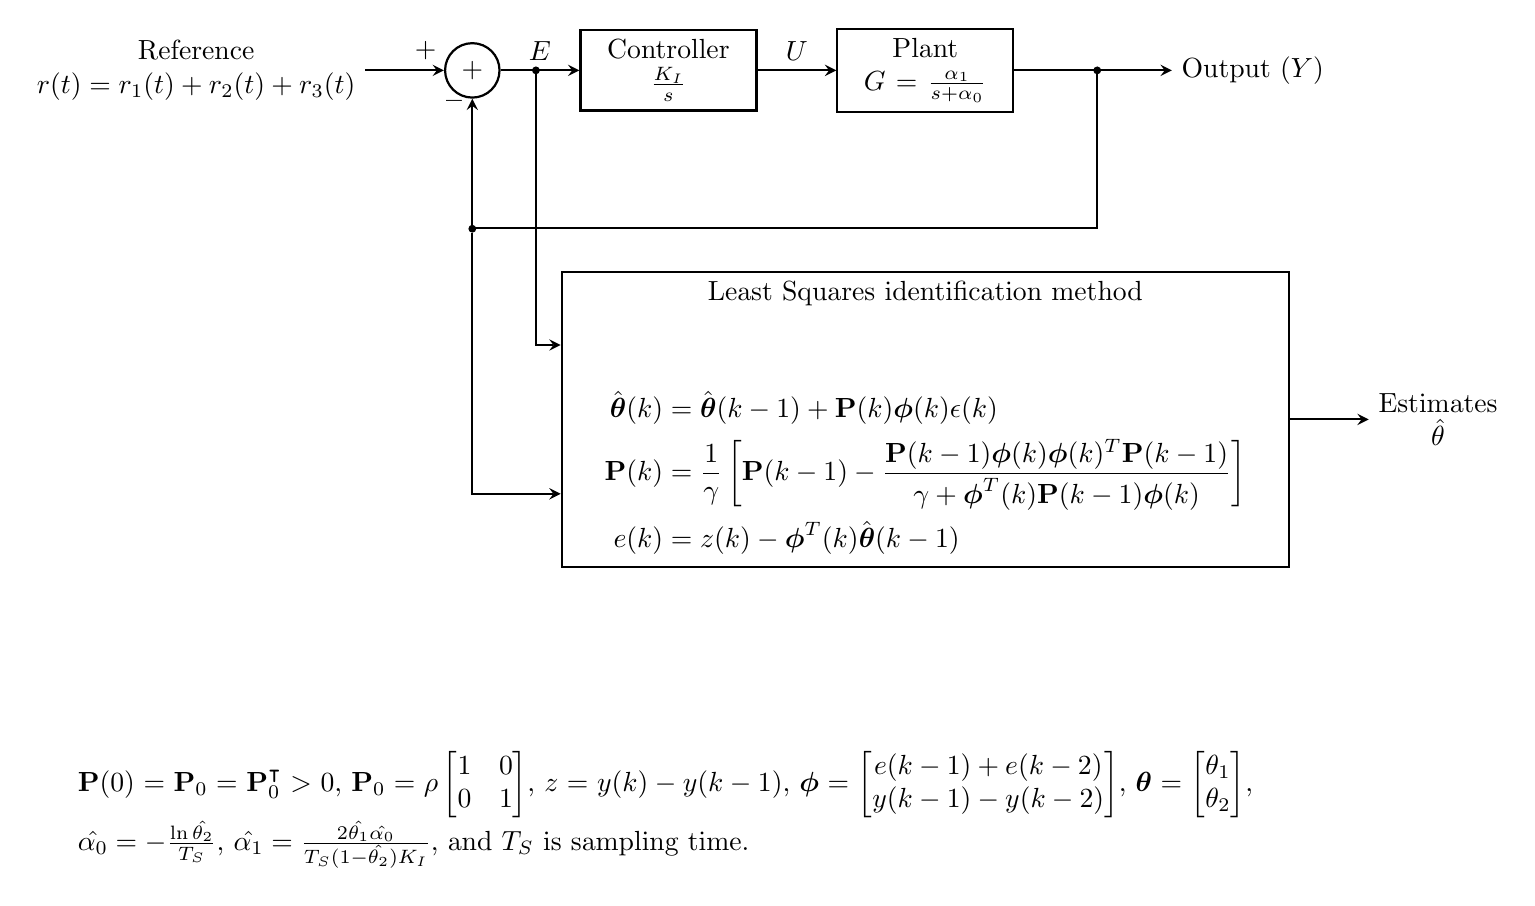
\begin{tikzpicture}[node distance = 10mm, auto]
		\node (Reference) [align=center] {Reference\\$r(t)=r_1(t)+r_2(t)+r_3(t)$};
		\node (SummingPoint) [draw,circle, thick, right = of Reference]  {+};
		\node (Control) [block, text width = 2cm, right = of SummingPoint] {Controller\\$\frac{K_I}{s}$};
		\node (ControlLeft) [support, left = of Control, left = 0.5cm, fill,circle,scale=0.3] {};
		\node (Plant) [block, text width = 2cm, right = of Control] {Plant \\$G=\frac{\alpha_1}{s+\alpha_0}$};
		\node (PlantRight) [support, right = of Plant, right = 1cm, fill,circle,scale=0.3] {};
		\node (Output) [right = of Plant, right = 2cm] {Output ($Y$)};
		\node (Identification) [block, text width = 9cm, below = 2cm of Plant] {Least Squares identification method
			\\[0.3cm]
			\begin{align}
				\hat{\boldsymbol{ \theta}}(k) &=\hat{\boldsymbol{ \theta}}(k-1)+\mathbf{P}(k)\boldsymbol{ \phi}(k)\epsilon(k) \nonumber\\ 
				\mathbf{P}(k) &=\dfrac{1}{\gamma}\left[\mathbf{P}(k-1)-\dfrac{\mathbf{P}(k-1)\boldsymbol{ \phi}(k)\boldsymbol{ \phi}(k)^{T}\mathbf{P}(k-1)}{\gamma+\boldsymbol{ \phi}^{T}(k)\mathbf{P}(k-1)\boldsymbol{ \phi}(k)}\right] \nonumber\\ 
				e(k) &=z(k)-\boldsymbol{ \phi}^{T}(k)\hat{\boldsymbol{ \theta}}(k-1) \nonumber 
			\end{align}

		};
		\node (OutputTapingPoint) [support, below = of SummingPoint, below = 1.6cm, fill,circle,scale=0.3] {};
		\node (CapValues) [right = of Identification, right = 1cm, align=center] {Estimates\\$\hat{\theta}$};
		\draw [arrow] (Reference) -- node[anchor=south west]{+}(SummingPoint);
		\draw [arrow] (SummingPoint) -- node[anchor=south]{$E$}(Control);
		\draw [arrow] (Control) -- node[anchor=south]{$U$}(Plant);
		\draw [arrow] (Plant) -- (Output);
		\draw [arrow] (PlantRight) -- +(0, -2) -| (SummingPoint) node[below = 2mm, anchor=north east]{\bf\textendash};
		\path (Identification.west) -- (Identification.north west) coordinate[pos=0.5] (Identification1);
		\path (Identification.west) -- (Identification.north west) coordinate[pos=-0.5] (Identification2);
		\draw [arrow] (ControlLeft) |- (Identification1);
		\draw [arrow] (OutputTapingPoint) |- (Identification2);
		\draw [arrow] (Identification) -- (CapValues);
		\node (Equation000) [text width = 15cm, below = 8cm of Control, align = left] {
			$\textbf{P}(0) = \textbf{P}_0 = \textbf{P}_0^\intercal>0$, $\textbf{P}_0 = \rho
			\begin{bmatrix}
			1 & 0 \\
			0 & 1
			\end{bmatrix}$,
			$z = y(k) - y(k-1)$,
			$\boldsymbol{\phi} = \begin{bmatrix}
			e(k-1) + e(k-2) \\
			y(k-1) - y(k-2)
			\end{bmatrix}$,
			$\boldsymbol{\theta} = \begin{bmatrix}
			\theta_1 \\
			\theta_2
			\end{bmatrix}$,
			$\hat{\alpha_0} = -\frac{\ln{\hat{\theta_2}}}{T_S}$,
			$\hat{\alpha_1} = \frac{2\hat{\theta_1}\hat{\alpha_0}}{T_S(1-\hat{\theta_2})K_I}$, and $T_S$ is sampling time.
		};
		\end{tikzpicture}
		\caption{Parameter estimation of a first order system with integral controller}
		\label{Fig:IdentificationWithIntegralController}
	\end{figure}
	
	%\bibliographystyle{apacite}%unsrtnat}
	%\bibliographystyle{spbasic}      % basic style, author-year citations
	%\bibliographystyle{spmpsci}      % mathematics and physical sciences
	%\bibliographystyle{spphys}       % APS-like style for physics
	%\bibliographystyle{ieeetr}
	%\bibliography{refs}
\end{document}